\chapter{Analysis of Existing Syntactic and Semantic Analysers}
\label{ch:current-analyzers-analysis}

In the Related Work (\cref{ch:retalted-work}) some ShEx tools were explained. This section will detail more
those tools that provide any kind error and warning detection and reporting. After, we will detail the points
that we think can be enhanced.

Before start the analysis we must define a methodology in order to be able to make an even analysis for all
existing tools.

\section{Methodology}
To evaluate existing systems from a neutral point of view we will use the ShEx specification as the basis.
However, this specification does not cover all possible cases, in particular it leaves most semantic restrictions
to the choice of the specific implementation.

Therefore, as regards this evaluation, when a semantic option not contemplated by the specification is proposed,
the option that favours the security of the language will be chosen. For example. If the specification did not say
anything about whether a variable can be redefined and we had to take an option, we will always choose not, so that
the language is as safe as possible and does not lead to errors.

The unique syntactic restrictions applied is:
\begin{itemize}
  \item In the last triple constraint of a set expression the trailing semicolon it is optional but recommended.
\end{itemize}

The semantic restrictions that have been applied are listed below.
\begin{itemize}
  \item Overwriting of prefixes is not allowed.
  \item Overwriting of the base is not allowed.
  \item Overwriting of the start shape is not allowed.
  \item Overwriting of shapes is not allowed.
  \item All references must exist within the scope of the schema.
\end{itemize}

In addition, in this evaluation we will use different test cases for each system, specifically the test cases
correspond to each element of the ShEx micro Compact grammar. Remember that the elements that this grammar has
are: \textit{definition of prefixes}, \textit{definition of the base}, \textit{definition of the start shape} and
\textit{definition of shapes}.
To others within the previous elements you will also find references to prefixes, the base and other shapes.
Therefore we will test all these elements in their syntactic and semantic aspects. \cref{fig:shexc-micro-errors}
shows some examples of this errors.

\begin{figure}
    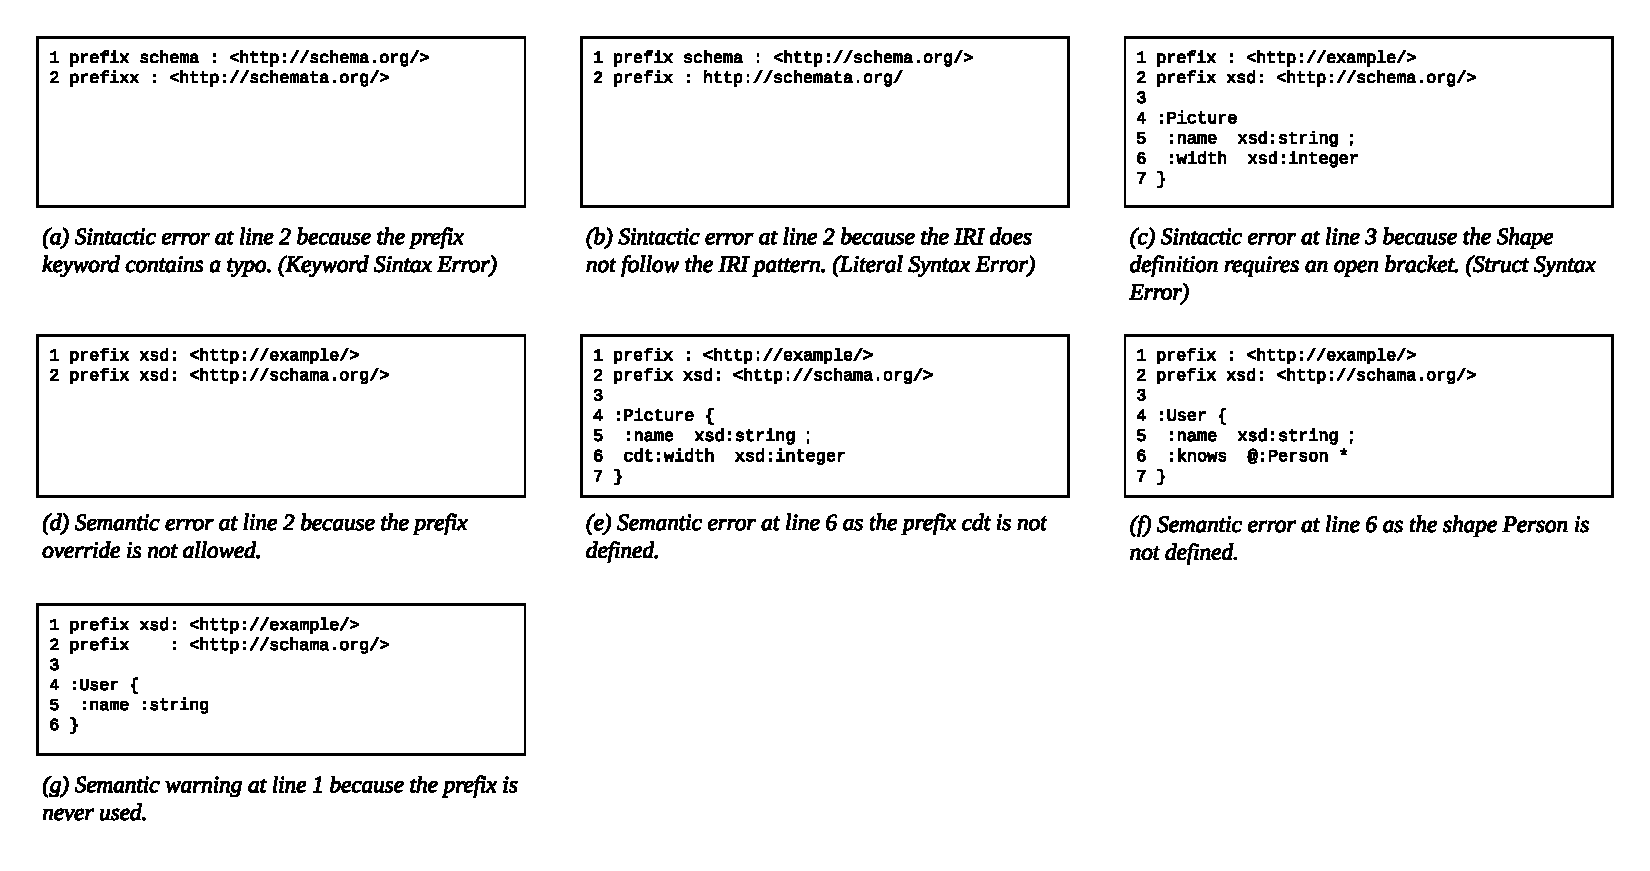
\includegraphics[width=\textwidth]{images/shexc-micro-bad-examples.pdf}
    \centering
    \caption[Examples of ShEx micro Compact Syntax code containing syntactic and semantic errors or warnings]{Examples of ShEx micro Compact Syntax
    code containing errors.}
    \label{fig:shexc-micro-errors}
  \end{figure}

\section{Syntactic Analysers}
According to \cite{floyd1963syntactic} we consider a Syntactic Analyzer a piece of software capable of parse, generate
a parse tree and detect and retorting syntactic warnings and errors.

Therefore in this category we would include \textbf{Shaclex}, \textbf{ShEx.js}, \textbf{YASHE} and \textbf{VS Code Plugin}.
\cref{tb:sintactic-errors} shows a comparison between the analysed tools.

Some comments to be made about the results obtained are that although we get an error for syntactic errors,
the quality of the error is more or less always the same. For example for the fragment \texttt{prefixx xsd: <http://example/>}
where we introduced an error at the keywork \texttt{prefix} by adding an extra \texttt{x} the error obtained is: \texttt{This line is invalid. Expected: PNAME\_NS.}

To our point of view this error message nor is not correct because it does not provide the user enough information to fix the schema.

Then also it is important to remark that during this analysis we encounter other syntactic problems that where not detected by tools like Shaclex,
an example is that properties like \texttt{schema:rdf@:name} \textit{(which is not a valid IRI)} are accepted without errors.

\begin{table}
  \centering
  \caption{Detection of the different syntactic errors by the current existing ShEx tools that syntactically analyse the
  shape expressions.}
  \label{tb:sintactic-errors}
  \resizebox{\textwidth}{!}{\begin{tabular}{lcccccccc} 
    \hline\hline
                   & \multicolumn{8}{c}{Sintactic Errors}                                                                                                                                                                                                                                                                                                                          \\ 
    \hline
    Analyzers      & \multicolumn{1}{l}{Prefix Definition} & \multicolumn{1}{l}{Base Definition} & \multicolumn{1}{l}{Start Shape} & \multicolumn{1}{l}{Shape Definition} & \multicolumn{1}{l}{Prefix Reference} & \multicolumn{1}{l}{Base Reference} & \multicolumn{1}{l}{Shape Reference} & \begin{tabular}[c]{@{}c@{}}Recomends Semicolon\\Last Triple Constraint\end{tabular}  \\ 
    \hline
    Shaclex        & Yes                                   & Yes                                 & Yes                             & Yes                                  & Not completly                        & Yes                                & Yes                                 & No                                                                                   \\
    ShEx.js        & Yes                                   & Yes                                 & Yes                             & Yes                                  & Yes                                  & Yes                                & Yes                                 & No                                                                                   \\
    YASHE          & Yes                                   & Yes                                 & Yes                             & Yes                                  & Yes                                  & Yes                                & Yes                                 & No                                                                                   \\
    VS Code Plugin & Yes                                   & Yes                                 & Yes                             & Yes                                  & Yes                                  & Yes                                & Yes                                 & No                                                                                   \\
    \hline
    \end{tabular}}
\end{table}

\section{Semantic Analysers}
As Semantic Analysers we will only consider those tools that validate the semantics of the language, in this section we
include the validation of references like prefixes and shapes. The tools that claim to support this validations are
\textbf{Shaclex}, \textbf{ShEx.js}, and \textbf{YASHE}. \cref{tb:semantic-errors} shows a comparison between the analysed tools.

From the obtained results we have to point that most of the tools opted for an open policy when talking about language semantics. From our
point of view this have its advantages and its drawbacks. But this only affects to the override policy. All of the tools should
implement the non existing references validation and most of them only focus on prefixes definition with the exception of
YASHE which does the checking of the shape reference but the error message sometimes is not completely accurate.

It it also remarkable that none of the tools performs a deeper analysis so there is no detection of unused resources, therefore
no warnings are generated by none of the existing tools.

\begin{table}
  \centering
  \caption{Detection of the different semantic errors by the current existing ShEx tools that semantically analyze the
  shape expressions.}
  \label{tb:semantic-errors}
  \resizebox{\textwidth}{!}{\begin{tabular}{lccccccc} 
    \hline\hline
                   & \multicolumn{7}{c}{Semantic Errors}                                                                                                                                                                                                                                                                                                                                                 \\ 
    \hline
    Analyzers      & \multicolumn{1}{l}{Prefix Override} & \multicolumn{1}{l}{Base Override} & \multicolumn{1}{l}{Start Shape Override} & \multicolumn{1}{l}{Shape Override} & \begin{tabular}[c]{@{}c@{}}Non Existing\\Prefix Reference \end{tabular} & \begin{tabular}[c]{@{}c@{}}Non Existing\\Base Reference \end{tabular} & \begin{tabular}[c]{@{}c@{}}Non Existing\\Shape Reference \end{tabular}  \\ 
    \hline
    Shaclex        & No                                  & No                                & No                                       & No                                 & Yes                                                                     & -                                                                     & No                                                                      \\
    ShEx.js        & No                                  & No                                & No                                       & No                                 & Yes                                                                     & -                                                                     & No                                                                      \\
    YASHE          & No                                  & No                                & No                                       & No                                 & Yes                                                                     & -                                                                     & Yes\footnote{When in the shape reference the prefix is the reference that is not right it still indicates that the shape is the one not existing.}                                                                     \\
    \hline
    \end{tabular}}
\end{table}

\section{Possible Enhancements}\label{sec:anal-enhacements}
Previous sections show the current state of the existing tools, their capabilities and their lacks.
With all that information we propose a list of enhancements that can be done to improve the error and warning detection
As seen in previous sections there's work that can be done to improve the existing ecosystem of tools. We have identified the following aspects
that will benefit end users:

\begin{enumerate}
    \item \textbf{Enhancement of error messages \cite{heeren2005top}.} Existing error messages, originated both by syntactic or semantic errors do not offer information about
    the exact place that originates the error nor a processed description nor possible solutions.

    \item \textbf{Creation of a new type of error messages with lower importance called warnings.} Currently systems do not analyse if declared resources are
    used and therefore there is no need to generate warnings. We propose to not only fully analyse the resources to detect non-used ones but also the creation
    or error messages with lower importance like warnings that can be used to offer more information to the end user.

    \item \textbf{Detection of override definitions.} Most of the existing tools prefer not to detect when a definition is being overridden, we propose to detect those
    situations and treat definitions as fixed values.

    \item \textbf{Detection of undefined references.} Some tools detect some broken references, we propose to enchase this situation and take that behaviour to
    other elements like shape references.

    \item \textbf{Detection of unused resources.} Related to the second point sometimes new users copy and paste old code which ends with lots of unused code,
    we propose a system that detects those situations and suggest to remove that unused code.

    \item \textbf{Detection of multiple errors / warnings at once.} Most of the current analysers only provide information about the first error they find,
    this means that if we have a scheme with multiple errors or warnings, only the first one will be shown to us and we will not be able to see the next one
    until we solve the previous one. 
\end{enumerate}